\section{Konzept}
Hier wird ein Konzept mit Mock Ups und Architektur entstehen
\subsection{Priorisierung der Erfassungsmöglichkeiten}
\sectionauthor{Lukas Seemann}
Nachdem im vorherigen Kapitel verschiedene Möglichkeiten vorgestellt wurden, mit denen Anzeichen von Emotionen bei Menschen gemessen werden können, werden nun diese Möglichkeiten priorisiert. In der folgenden Tabelle (Tabelle 1) ist die Priosierung abgebildet. \newline
\begin{table}[h]
	\centering
	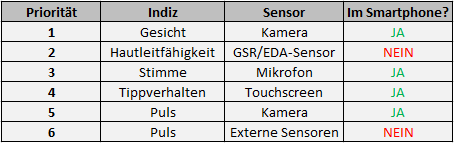
\includegraphics[width=14cm]{Bilder/prio.png}
	\caption[Priorisierung der Erfassungsmöglichkeiten]{Priorisierung der Erfassungsmöglichkeiten}
\end{table}%
\newline In der ersten Spalte ist die Priorität dargestellt. Je niedriger die Zahl ist, desto höher ist die Erfassungsmöglichkeit priorisiert. Die Möglichkeiten werden in der Reihenfolge der hier dargestellten Priorisierung thematisiert und letzten Endes in den Prototyp der mobilen Applikation integriert, um Daten zu erfassen. Je nachdem wie viel Zeit die einzelnen Features benötigen, können mehr und mehr Möglichkeiten der Datenerfassung in die App eingebaut werden, wenn sie noch im Zeitrahmen der Studienarbeit umsetzbar sind. Bei den einzelnen Möglichkeiten werden das Indiz, anhand dessen Rückschlüsse auf eine Emotion gemacht werden kann, und ein Sensor, der Daten zum Indiz für die App erfassen soll, aufgelistet. In der letzen Spalte ist festgehalten, ob der benötigte Sensor in den meisten aktuellen Smartphones bereits enthalten ist oder nicht. \newline
Die höchste Priorität hat das Indiz der Hautleitfähigkeit, die mithilfe von GSR- beziehungsweise EDA-Sensoren erfasst werden kann. Diese Art von Sensoren befinden sich nicht in handelsüblichen Smartphones, weshalb man hierzu externe Sensoren mit dem Handy verbinden muss. \newline
...

\subsection{Datenerfassung}
\subsection{Auswertung}
\subsection{Entscheidungsalgorithmus}
\sectionauthor{Torben Brenner}
Ziel der Anwendung ist es, basierend auf zuvor aufgenommenen Daten eine Entscheidung zu fällen, welche Emotion der Nutzer der 
Anwendung aktuell empfinden könnte. Die Entscheidung muss dabei die verschiedenen Ergebnisse der Auswertungsebene einbeziehen
und aus diesen auf eine Emotion schließen. Deshalb muss eine Einheitliche Datenstruktur entwickelt werden, über die die Auswertungsebene
die Daten zur Verfügung stellt. \\
Die Entscheidung könnte hierbei über ein \textit{Scoring} entstehen. Dieses \textit{Scoring} müsste dabei auf der Auswertungsebene stattfinden, 
wobei jeder der Auswertungsalgorithmen ein \textit{Scoring} für die verschiedenen Emotionen angeben muss. Am Ende könnten z. Bsp. die verschiedenen 
\textit{Scorings} addiert und die Emotion mit dem höchsten \textit{Scoring} ausgewählt werden.